% !Mode:: "TeX:UTF-8"
% Author: Zhengxi Tian
% Email: zhengxi.tian@hotmail.com

\chapter{绪论}\label{ch:introduction}
% \footnote{http://www.opensubtitles.org}

\section{课题研究背景}\label{sec:research_background}
% Task-Oriented and Chat-Oriented.
早期的对话系统的用途主要是帮助用户用自然语言完成某项任务,比如技术支持(Technical Support),预订机票、预订餐馆的座位、查询航班等。这一类系统又被称为任务导向的系统(Task-Oriented),其实现技术包括关键词匹配、规则和模板以及对话状态追踪(Dialogue State Tracking)等等,往往需要大量人工标注的数据。这些系统只能处理特定领域内的对话,不能回答开放性问题,用途局限于特定领域
\upcite{
DBLP:journals/corr/SerbanLCP15,
DBLP:journals/corr/VinyalsL15,
DBLP:conf/acl/ShangLL15}。

随着在线聊天的流行,社交媒体和互联网论坛积累了大量的聊天语料数据,具有代表性的社交媒体和论坛有Twitter,Reddit和微博。大量的数据使人们可以构建数据驱动的(Data-Driven),开放领域(Open-Domain)的对话系统\upcite{Ritter:2011:DRG:2145432.2145500}。这种系统能根据对话的上下文和用户的提问产生语义相关的回答,用途有娱乐、语言学习工具和陪伴\upcite{DBLP:conf/aaai/SerbanSBCP16}等等。该领域主要考察二人对话,两人聊天的历史记录称为上下文(context),记为$c$;当前说话的人说出的话语称为消息(message),记为$m$;另外一个人对该消息的回复称为响应(response),记为$r$。$c,m,r$三者的关系如图~\ref{fig:context_message_response}所示。系统的输入是$c,m$,输出是$r$,也就是把对话的上下文和消息映射为响应,这个问题被称为对话响应生成(Conversation Response Generation)。

\begin{figure}[H]
    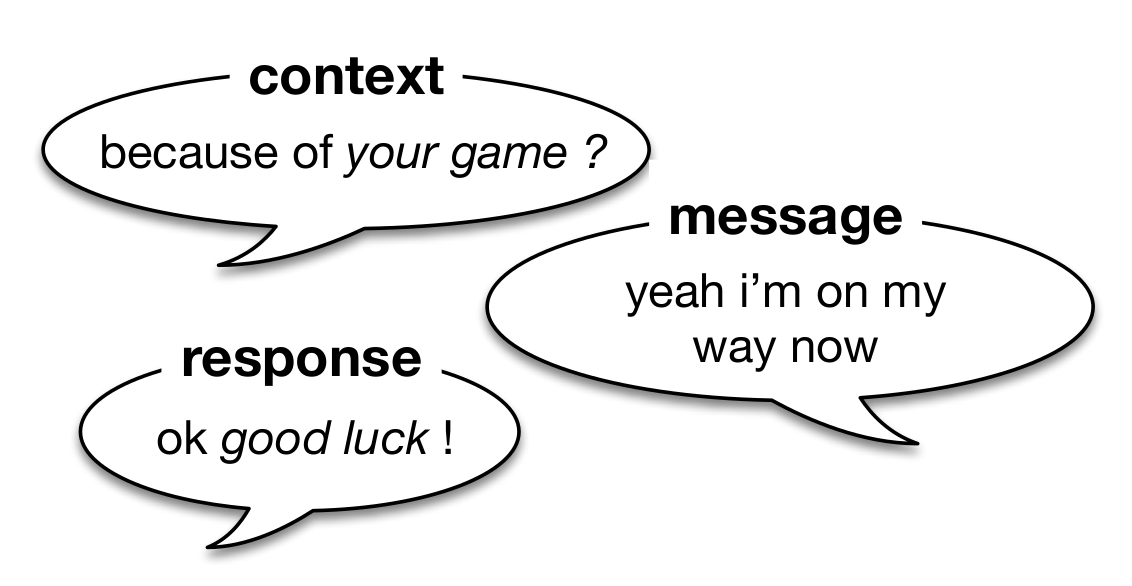
\includegraphics[width=0.6\textwidth]{figure/context_message_response.png}
    \centering
    \caption{上下文,消息和响应的关系\upcite{DBLP:journals/corr/SordoniGABJMNGD15}}
    \label{fig:context_message_response}
\end{figure}

% Retrieval and Generative.
对话系统又可以分为生成式对话系统(Generative System)和检索式对话系统(Retrieval-Based System)\upcite{DBLP:journals/corr/SerbanLCP15}。
如果一个系统能生成训练集里没有的句子,就把它称为“生成式系统”\upcite{DBLP:conf/emnlp/LiuLSNCP16}。
两种系统的区别在于:生成式系统以输入句子为条件,把条件概率最大的句子作为输出。
由于搜索空间过于庞大,在实际中通常采用某种启发式搜索方法,如集束搜索(Beam Search),贪婪搜索(Greedy Search)
和随机取样(Random Sample)。
设$X$为输入句子,$Y$为输出句子,$U$是全部句子的集合,生成式模型的一般表示为:
\begin{align}
    Y = \text{argmax}_{Y\in U} \left(p(Y|X)\right)
\end{align}
检索式系统根据输入句子从一个数据库$D$中检索输出句子。
$D$通常由人类撰写的语句组成,并且足够大,使得输出句子不容易重复。
系统通过某种打分机制,如词频-逆文档频率(Term Frequency-Inverse Document Frequency,TF-IDF)
对数据库中的候选句子进行打分,并把得分较高的候选作为输出:
\begin{align}
    Y = \text{argmax}_{Y\in D} Score(Y, X)
\end{align}
可见,生成式系统和检索式系统的根本区别在于获得输出句子的机制不同。
这两种方法各有优劣:检索式模型的输出没有语法错误且和输入的相关度比较高,但是不能生成新句子;
生成式的模型能针对输入生成个性化的输出且系统高度灵活\upcite{DBLP:conf/acl/ShangLL15},但是容易生成过短的句子\upcite{
DBLP:journals/corr/KannanV17}。
在实际环境中,通常将它们作为模型联合体(Model Ensemble)使用\upcite{DBLP:journals/corr/SongYLZZ16},
而检索式系统也经常作为生成式系统的基线系统与之比较\upcite{
DBLP:conf/acl/ShangLL15,
DBLP:journals/corr/SordoniGABJMNGD15}。

% RNN, Seq2Seq and Embedding
生成式模型的流行得益于自然语言处理领域发展的一系列基础技术,包括
为单词提供平滑特征的词嵌入(Word Embedding)\upcite{
DBLP:journals/jmlr/BengioDVJ03,
DBLP:journals/corr/abs-1301-3781,
DBLP:conf/emnlp/PenningtonSM14};
能对变长序列建模的循环神经网络语言模型(Recurrent Neural Networks Language Model,RNNLM)\upcite{DBLP:conf/interspeech/MikolovKBCK10};
易于训练,能避免梯度消失问题的循环门单元,如长短期记忆单元(Long Short-Term Memory,LSTM)
\upcite{DBLP:journals/neco/HochreiterS97}和门循环单元(Gated Recurrent Unit,GRU)\upcite{DBLP:conf/emnlp/ChoMGBBSB14};
以及基于编解码器结构和RNN的序列到序列框架(Sequence to Sequence Framework,Seq2Seq)\upcite{
DBLP:conf/nips/SutskeverVL14,
DBLP:conf/emnlp/ChoMGBBSB14},图~\ref{fig:Seq2Seq}是Seq2Seq的模型结构图。

% Chatbot in Seq2Seq.
Seq2Seq框架在自然语言处理的多项任务上都超过了之前的方法,因此被广泛应用到对话生成领域。
最早把Seq2Seq用到对话生成领域的是Vinyals等人\upcite{DBLP:journals/corr/VinyalsL15},
他们在OpenSubtitles\upcite{DBLP:conf/lrec/LisonT16}
上训练的模型能回答简单的常识问题,
并且比基于规则的系统CleverBot\footnote{http://www.cleverbot.com/}获得了更高的人类评价得分。
% ------------------------------------- %
Li等人提出了一系列基于Seq2Seq框架的对话系统,包括
利用最大互信息(Maximum Mutual Information,MMI)增加输出多样性的目标函数\upcite{DBLP:conf/naacl/LiGBGD16},
在解码器端(Decoder)加入说话人身份信息(Speaker ID)以达到输出的人格一致性(Persona Coherence)
\upcite{DBLP:journals/corr/LiGBGD16}以及利用对抗生成网络(Generative Adversarial Networks,GAN)
\upcite{DBLP:journals/corr/GoodfellowPMXWOCB14}使系统输出和人类输出难以分辨\upcite{DBLP:conf/emnlp/LiMSJRJ17}
等等。
% ------------------------------------- %
Serban等人把Sordoni等人提出的用于查询建议(Query Suggestion)的
层级循环编解码器(Hierarchical Recurrent Encoder-Decoder,HRED)\upcite{DBLP:conf/cikm/SordoniBVLSN15}应用到对话生成领域, 提出了能捕捉对话的层级结构的HRED模型\upcite{DBLP:conf/aaai/SerbanSBCP16}。
基于HRED,Serban等人又提出了利用随机潜变量(Stochastic Latent Variable)增加对话多样性的Variational Hierarchical Recurrent Encoder-Decoder,即VHRED\upcite{DBLP:journals/corr/SerbanSLCPCB16};
以及加入了多层次抽象信息的多精度循环网络(Multiresolution Recurrent Neural Networks,MultiRNN)
\upcite{DBLP:conf/aaai/SerbanKTTZBC17}。
% --------- China's researches ----------- %
在国内,Shang等人研究了微博数据集上的短文本对话生成问题(Short-Text-Conversation,STC),
提出了以GRU为门单元的编解码器模型(Neural Response Machine,NRM)\upcite{DBLP:conf/acl/ShangLL15},
并在人类评价上取得了比检索式系统和翻译式系统\upcite{Ritter:2011:DRG:2145432.2145500}更好的成绩。
Chen Xing等人向Seq2Seq加入了从预训练LDA模型中获取的主题词(Topic Words)并提出了Topic-Aware Seq2Seq
\upcite{DBLP:conf/aaai/XingWWLHZM17}。由于篇幅有限,不能一一介绍。

\begin{figure}[H]
    \centering
    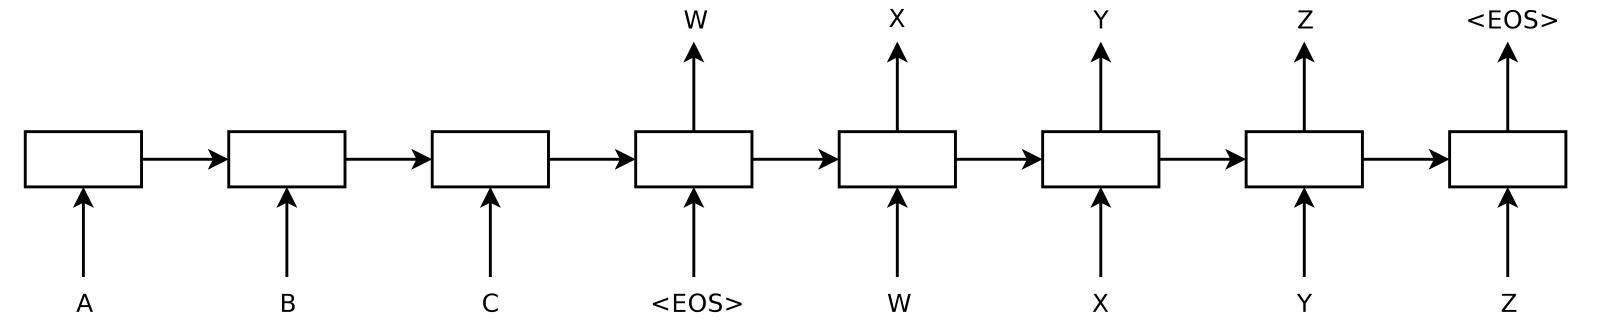
\includegraphics[width=0.8\textwidth]{figure/Seq2Seq.png}
    \caption{Seq2Seq框架图\upcite{DBLP:conf/nips/SutskeverVL14}}
    \label{fig:Seq2Seq}
\end{figure}

\section{课题研究意义}\label{sec:research_meaning}
% 存在的问题:1. 评估模型的困难性。2. 容易生成Naive响应。
% A long-standing problem in this field is the difficulty of evaluating the generated responses.
生成式对话系统目前有两个难题:一是评价系统生成的响应的困难性\upcite{
DBLP:conf/emnlp/LiuLSNCP16,
DBLP:conf/acl/ShangLL15,
DBLP:conf/emnlp/LiMRJGG16,
DBLP:conf/acl/GalleyBSJAQMGD15,
DBLP:conf/acl/LoweNSABP17};
二是如何避免生成单调的响应
\upcite{
    DBLP:conf/naacl/LiGBGD16,
    DBLP:journals/corr/LiMJ17a,
    Ritter:2011:DRG:2145432.2145500,
    DBLP:journals/corr/SordoniGABJMNGD15,
    DBLP:conf/aaai/SerbanSBCP16}。
对第一个难题的一个普遍解释是,和机器翻译相比,对话生成的输出具有更高的熵(Entropy)。
在对话的场景下,给定一个消息,往往存在大量合理的响应,这些响应和参考响应(Ground Truth)的语义可能完全不一样,
并且彼此有着各异的语义。

\begin{table}[H]
    \centering
    \caption{合理的响应不唯一\upcite{DBLP:conf/aaai/TaoMZY18}}
    \label{tab:multiple_valid_responses}
    \begin{tabular}{rl}
        \toprule
        \textbf{Query:} & 为什么不领养一个? \\
        & Why not adopt one? \\
        \textbf{Groundtruth:} & 我也想领养,但是不好找 \\
        & I hope so, but it's hard to find one \\
        \midrule
        \textbf{Candidate 1:} & 恩,我已经在朋友中找了 \\
        & I'm looking for one from my friends \\
        \textbf{Candidate 2:} & 巴比伦是稀有品种 \\
        & Pappilon is a rare breed \\
        \textbf{Candidate 3:} & 可以哈,谢谢你的建议 \\
        & OK, thank you for your advice \\
        \bottomrule
    \end{tabular}
\end{table}

如表~\ref{tab:multiple_valid_responses}所示,合理的响应不唯一,这种固有的多样性决定了评价响应生成系统的困难。
Liu等人在\cite{DBLP:conf/emnlp/LiuLSNCP16}中研究了两类指标,分别是基于词重叠的指标(Word Overlap Based)
和基于词嵌入的指标(Embedding Based),并且发现这些指标在非技术性的Twitter数据集上和人类评价只有弱相关性,
在技术性的Ubuntu Dialogue Corpus\upcite{DBLP:conf/sigdial/LowePSP15}没有相关性。
Liu等人的工作为对话领域的自动评价指标的研究开辟了新的方向。

% ------- ADEM ------------ %
Lowe等人以自动化的图灵测试(Automatic Turing Test)为灵感,
提出了一个以VHRED为编码器,根据消息、参考响应和模型响应预测人类评分的模型,
称为自动化对话评价模型(Automatic Dialogue Evaluation Model,ADEM)\upcite{DBLP:conf/acl/LoweNSABP17}。
他们在新的数据和Liu的数据上评估了ADEM模型,发现它和人类评价的相关性在句子水平和系统水平都达到了很高水平。
% ------- AdverEval --------- %
Kannan等人在\cite{DBLP:journals/corr/KannanV17}中初步尝试了把GAN的方法应用到对话系统的自动评价中。
他们训练了一个鉴别器(Discriminator)来区分一个响应是来自系统还是来自人类,并且发现鉴别器能捕捉到基于Seq2Seq的模型
倾向于生成短句子和通用句子的缺点。
% ------ RUBER --------- %
在国内,Tao等人提出了基于神经网络和词嵌入的RUBER指标\upcite{DBLP:conf/aaai/TaoMZY18}。
该指标线性的结合了带参考的指标(Referenced Score)和不带参考的指标(Unreferenced Score),
并采用无监督的负采样(Negative Sampling)来训练模型,
在中文数据集豆瓣网\footnote{http://www.douban.com}上取得了很高的人类评价相关性。 % Correlation to Human Judgement
%这些研究进展的取得和Liu等人对自动化评价指标的实验和研究有着密切联系。

本课题延续Liu等人的工作,对自动评价指标进行深入研究。
Liu等人已经研究了评价指标与人类评价的相关性,并且发现了它们的弱点;
本文进一步研究了评价指标之间的相关性,以及模型的性能在不同数据集上的一致性。
虽然,目前大多数评价指标尚不能和人类评价一样准确的衡量系统的性能,
但是对它们性质的研究将有助于理解现有指标的弱点,进而有助于自动评价生成式对话系统的发展。

\section{课题研究内容}\label{sec:reseach_content}
本课题以\cite{DBLP:journals/corr/SerbanSLCPCB16}的实验中使用的三个模型LSTM,HRED,VHRED为基线,
扩展了\cite{DBLP:conf/emnlp/LiuLSNCP16}中考察的两类指标,
并在三个具有代表性的公开数据集:Ubuntu Dialogue Corpus,OpenSubtitles和LSDSCC\upcite{DBLP:conf/naacl/XuJLRWWWW18}上进行了实验。
尽管没有人类监督信号,但是我们对指标之间和模型之间的一致性分析还是取得了有意义的结论。
% 具体是什么结论,现在还不是很清楚。到时候实验一章写完之后,这里再修改。

\section{论文组织结构}\label{sec:paper_organization}
本文的组织结构如下:
第~\ref{ch:related_work}~章相关工作介绍了生成式对话领域中自动化指标的使用情况和研究现状;
第~\ref{ch:method}~章研究方法介绍了我们的实验方法以及实验涉及的指标、模型和数据集;
第~\ref{ch:experiment}~章实验结果与讨论详细展示了我们的实验配置、实验数据以及结论;
第~\ref{ch:conclusion}~章结论总结了本课题的研究成果,并展现了若干未来的研究方向。
% 某些写的笼统的地方,等实验结论出来之后,可以改的具体一些。
